\documentclass[UTF8]{ctexart}
\usepackage{geometry, CJKutf8}
\geometry{margin=1.5cm, vmargin={0pt,1cm}}
\setlength{\topmargin}{-1cm}
\setlength{\paperheight}{29.7cm}
\setlength{\textheight}{25.3cm}

% useful packages.
\usepackage{amsfonts}
\usepackage{amsmath}
\usepackage{amssymb}
\usepackage{amsthm}
\usepackage{enumerate}
\usepackage{graphicx}
\usepackage{subfigure}
\usepackage{multicol}
\usepackage{fancyhdr}
\usepackage{layout}
\usepackage{listings}
\usepackage{float, caption}

\lstset{
    basicstyle=\ttfamily, basewidth=0.5em
}

% some common command
\newcommand{\dif}{\mathrm{d}}
\newcommand{\avg}[1]{\left\langle #1 \right\rangle}
\newcommand{\difFrac}[2]{\frac{\dif #1}{\dif #2}}
\newcommand{\pdfFrac}[2]{\frac{\partial #1}{\partial #2}}
\newcommand{\OFL}{\mathrm{OFL}}
\newcommand{\UFL}{\mathrm{UFL}}
\newcommand{\fl}{\mathrm{fl}}
\newcommand{\op}{\odot}
\newcommand{\Eabs}{E_{\mathrm{abs}}}
\newcommand{\Erel}{E_{\mathrm{rel}}}

\begin{document}

\pagestyle{fancy}
\fancyhead{}
\lhead{张笑娟,3220101565}
\chead{数据结构与算法第五次作业}
\rhead{Nov.4th, 2024}

\section{remove函数的阐述}
    课本上不得不使用递归的原因在于findMin函数功能的缺失,findMin函数只支持返回最小节点的指针。minNode指针只是作为一个辅助指针,并不能真正指向最小节点,也不能对节点进行操作。
    而remove函数需要删除指定节点,因此在执行删除操作时不可避免地要进行递归操作,找到最小节点并删除,没有效率。
     
    所以,我们可以再定义一个detachMin函数,使其既可以找到最小节点,又可以执行删除操作。
    \begin{figure}[htbp] % [htbp]表示浮动选项,可以放置图片在合适位置
        \centering
        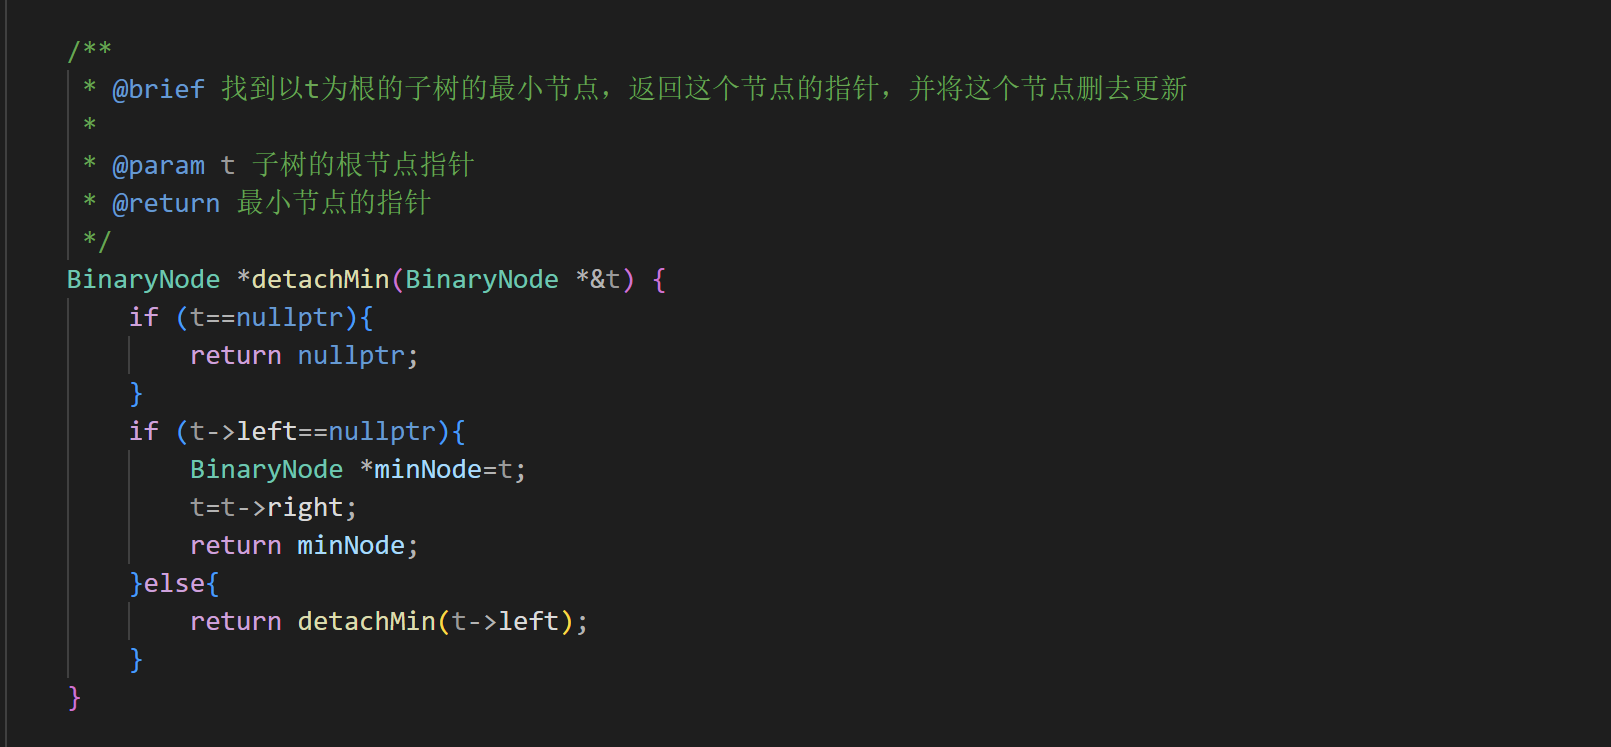
\includegraphics[width=0.8\textwidth]{detachMin.png} % 插入图片,设置宽度为页面宽度的80%
        \caption{detachMin函数} % 图片标题
        \label{1} % 给图片添加标签,便于引用
    \end{figure}

    然后再使用remove函数,调用detachMin函数找到最小节点并删除,同时将最小节点的值复制到当前节点。
    \begin{figure}[htbp] % [htbp]表示浮动选项,可以放置图片在合适位置
        \centering
        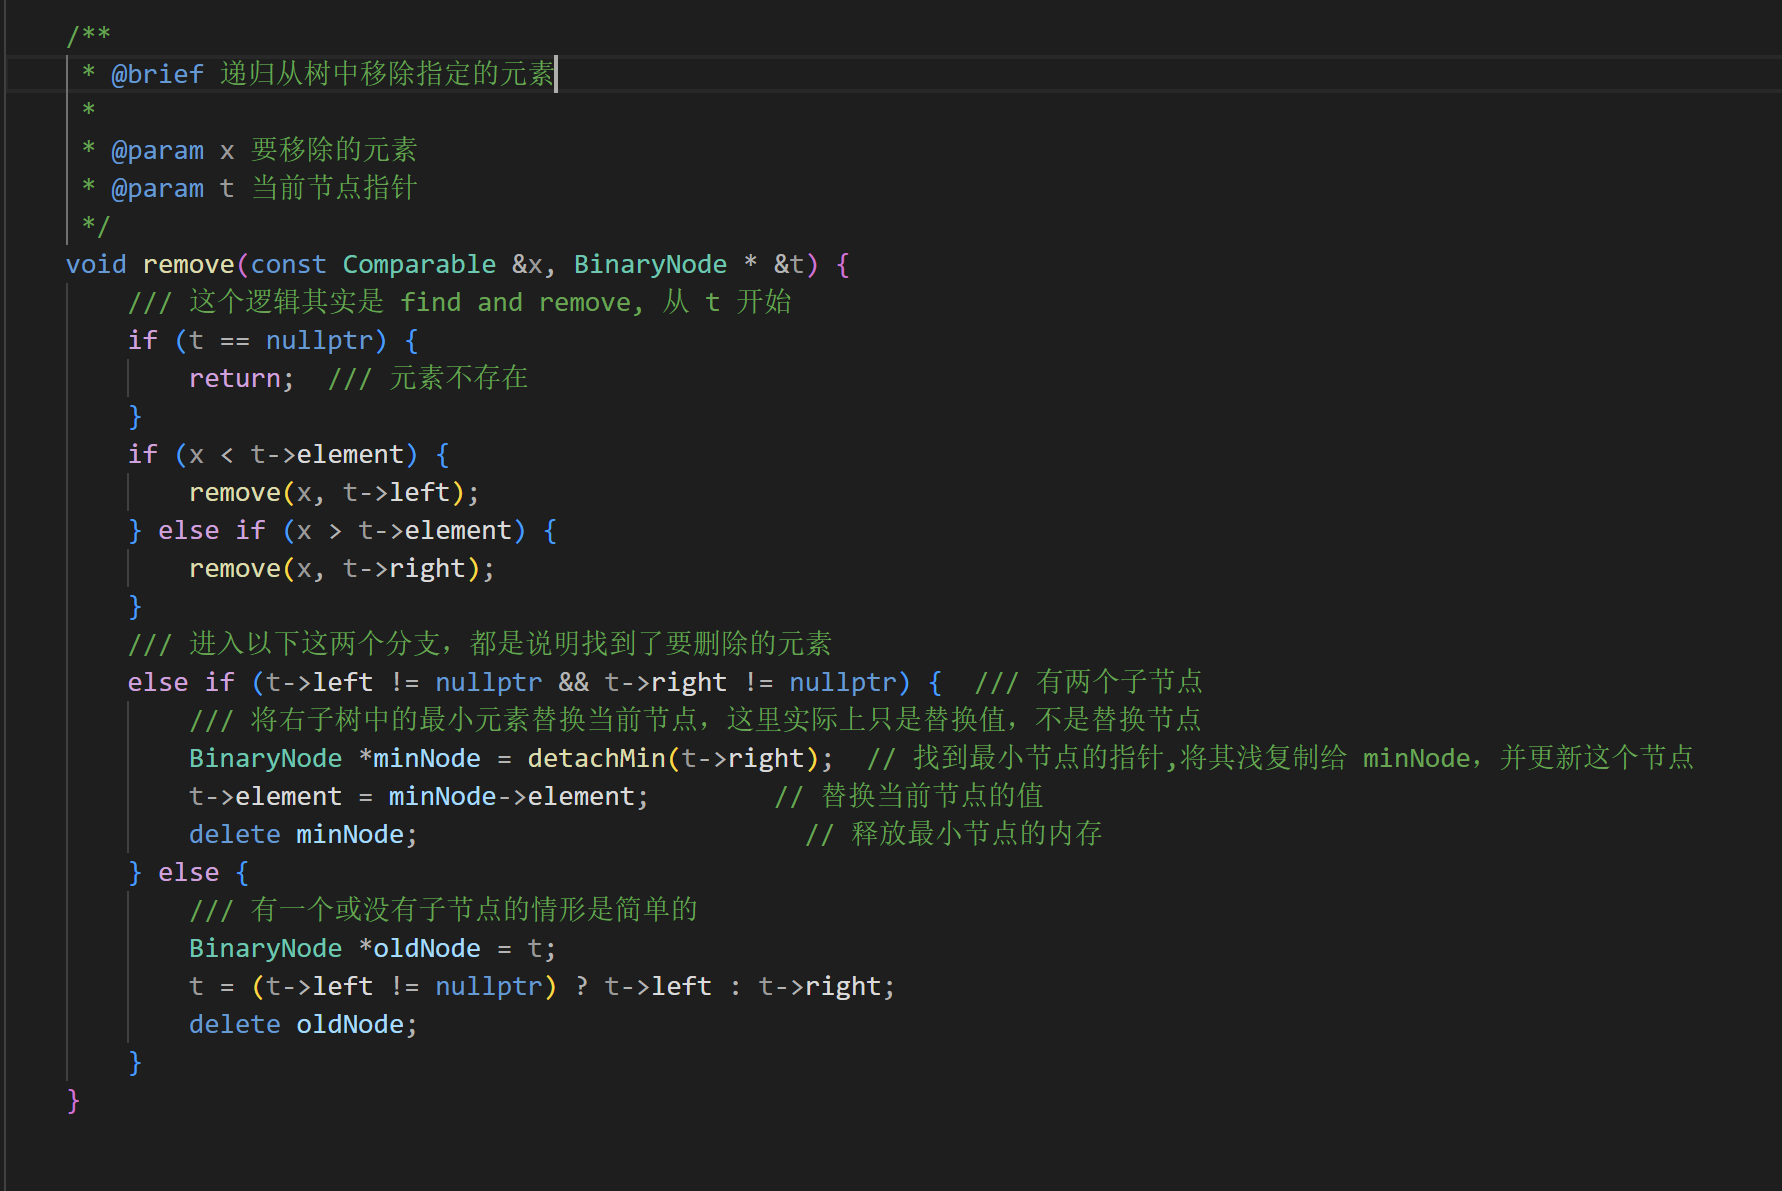
\includegraphics[width=0.8\textwidth]{remove.png} % 插入图片,设置宽度为页面宽度的80%
        \caption{remove函数} % 图片标题
        \label{2} % 给图片添加标签,便于引用
    \end{figure}


\section{测试的结果}   
 
    测试时采用老师的测试用例,输出结果正常。  
      
    \begin{figure}[htbp] % [htbp]表示浮动选项,可以放置图片在合适位置
        \centering
        \subfigure[]{
            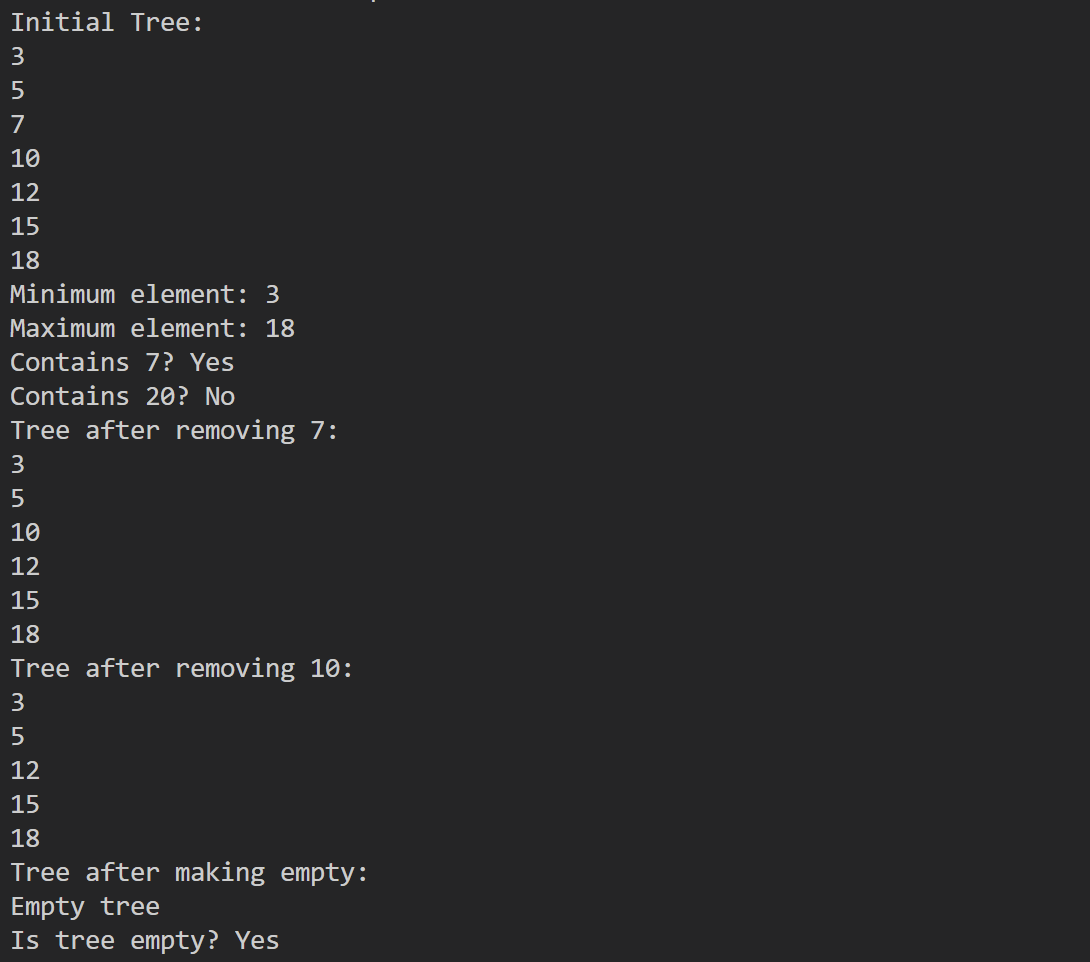
\includegraphics[width=0.65\textwidth]{result1.png}
            }
        \subfigure[]{
                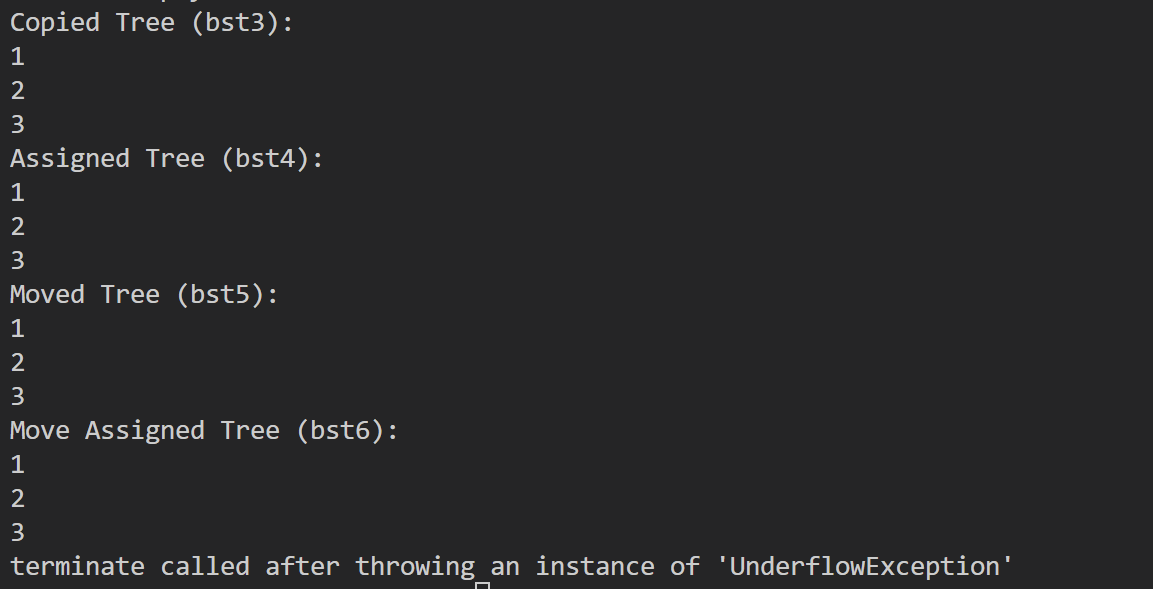
\includegraphics[width=0.65\textwidth]{result2.png}
        }
        \caption{测试结果} % 图片标题
        \label{3} % 给图片添加标签,便于引用
    \end{figure}
    可以看到,在删去10后输出为3 5 12 15 18,符合预期。

\end{document}

%%% Local Variables: 
%%% mode: latex
%%% TeX-master: t
%%% End: 